% Standalone Beamer deck. Diagrams and worked examples are original.
% Detailed derivations and evidence: ingersoll_2022_tracking.tex.
\documentclass[aspectratio=169,11pt]{beamer}
\usetheme{default}
\usepackage[T1]{fontenc}
\usepackage{lmodern,amsmath,amssymb,bm,booktabs,tabularx,tikz}
\usetikzlibrary{arrows.meta,positioning,fit}
\definecolor{ink}{HTML}{193549}
\definecolor{teal}{HTML}{007C83}
\definecolor{gold}{HTML}{AE690A}
\definecolor{quiet}{HTML}{607482}
\definecolor{paper}{HTML}{F7F9FA}
\setbeamercolor{normal text}{fg=ink,bg=white}
\setbeamercolor{structure}{fg=teal}
\setbeamercolor{frametitle}{fg=ink}
\setbeamercolor{title}{fg=ink}
\setbeamercolor{block title}{fg=ink,bg=teal!12}
\setbeamercolor{block body}{fg=ink,bg=teal!4}
\setbeamercolor{alerted text}{fg=gold}
\setbeamerfont{frametitle}{series=\bfseries,size=\Large}
\setbeamertemplate{navigation symbols}{}
\setbeamertemplate{itemize items}[circle]
\setbeamersize{text margin left=9mm,text margin right=9mm}
\hypersetup{colorlinks=true,urlcolor=teal}
\newcommand{\prov}{}
\newcommand{\evidence}[1]{\gdef\prov{#1}}
\newcommand{\takeaway}[1]{\vspace{0.3em}\begin{block}{What to remember}#1\end{block}}
\newcommand{\ms}{\mathrm{m\,s^{-1}}}
\newcommand{\sone}{\mathrm{s^{-1}}}
\newcommand{\Var}{\operatorname{Var}}
\newcommand{\Cov}{\operatorname{Cov}}
\newcommand{\paperlink}{\href{https://doi.org/10.1038/s41550-022-01774-0}{Ingersoll et al. (2022)}}
\newcommand{\repolink}{\href{https://github.com/ksr-ocean/jiram_catalog/blob/a6e3938e5c816583c49833791f7500e562acf155/docs/reports/tracking_pj4.md}{Repository PJ4 validation}}
\setbeamertemplate{footline}{%
 \leavevmode\hbox{%
 \begin{beamercolorbox}[wd=.90\paperwidth,ht=3ex,dp=1.5ex,leftskip=9mm]{normal text}
 \color{quiet}\tiny\prov
 \end{beamercolorbox}%
 \begin{beamercolorbox}[wd=.10\paperwidth,ht=3ex,dp=1.5ex,rightskip=6mm]{normal text}
 \hfill\color{quiet}\scriptsize\insertframenumber/\inserttotalframenumber
 \end{beamercolorbox}}}
\title{From cloud images to winds}
\subtitle{A pedagogical guide to the JIRAM approach\\of Ingersoll and colleagues}
\author{\texttt{jiram\_catalog} science notes}
\date{9 September 2026}

\begin{document}

\evidence{Reading guide: reported method, original teaching examples, repository evidence, proposed features.}
\begin{frame}[plain]
 \vspace{0.6cm}
 {\color{teal}\large JUPITER\quad/\quad CLOUD MOTION}
 \vspace{0.45cm}
 \titlepage
 \vspace{-0.5cm}
 \small\paperlink{}, \emph{Nature Astronomy}.
 \par\small Companion notes: \texttt{ingersoll\_2022\_tracking.tex}.
\end{frame}

\evidence{Original teaching framework. Detailed notes contain derivations and source locators.}
\begin{frame}{Follow one measurement through four steps}
 \begin{center}
 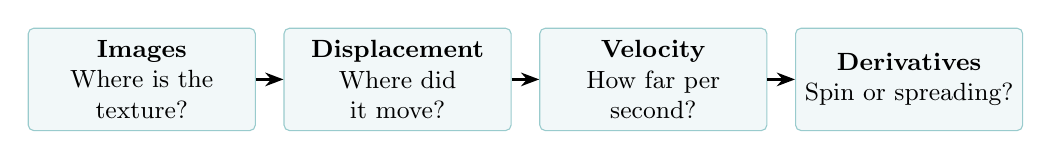
\begin{tikzpicture}[>=Stealth,
 box/.style={draw=teal!40,fill=teal!5,rounded corners=2pt,
 minimum height=1.3cm,text width=2.65cm,align=center,font=\small}]
 \node[box] (a) {\textbf{Images}\\Where is the texture?};
 \node[box,right=0.35cm of a] (b) {\textbf{Displacement}\\Where did it move?};
 \node[box,right=0.35cm of b] (c) {\textbf{Velocity}\\How far per second?};
 \node[box,right=0.35cm of c] (d) {\textbf{Derivatives}\\Spin or spreading?};
 \draw[->,thick] (a)--(b); \draw[->,thick] (b)--(c); \draw[->,thick] (c)--(d);
 \end{tikzpicture}
 \end{center}
 \vspace{0.6cm}
 Every step needs something extra: geometry, correspondence, timing, then
 spatial error control.
 \takeaway{A plausible arrow is the beginning of a wind measurement.}
\end{frame}

\evidence{Reported method: Ingersoll et al., Methods, Fig. 2 caption, Table 1. DOI linked on source slide.}
\begin{frame}{The experiment has a deliberately repeatable design}
 \small
 \begin{tabularx}{\linewidth}{@{}p{3.4cm}X@{}}
 \toprule
 Input & JIRAM M-band, 2 February 2017; four sets of twelve images.\\
 Mapping & SPICE/instrument geometry; polar orthographic map, 15 km pixels.\\
 Motion & Tracker3 correlation; $15\times15$ pixel patches, 225 km sides.\\
 Pair timing & n01--n03 and n02--n04; about 16 minutes, using actual image times.\\
 Sampling & 45 km vector spacing; native sampling varies from 22 to 14 km.\\
 Quality & Low-entropy patches masked; 256 brightness bins per patch.\\
 Diagnostics & Circulation/flux around 90, 180, 270, 360 km squares.\\
 \bottomrule
 \end{tabularx}
 \takeaway{A fixed recipe makes independent measurements comparable.}
\end{frame}

\evidence{Pairing design from Ingersoll et al., Methods and Fig. 2; timeline is an original schematic.}
\begin{frame}{Four image sets give two separate measurements}
 \begin{columns}[c]
 \column{0.59\textwidth}
 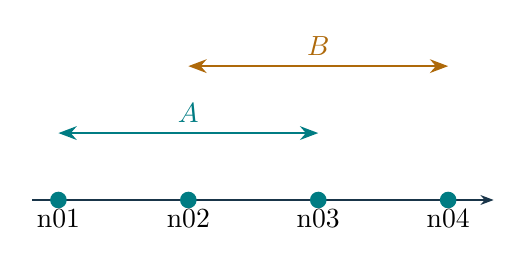
\begin{tikzpicture}[>=Stealth,x=1.65cm,y=0.85cm]
 \draw[->,ink] (-0.2,0)--(3.35,0);
 \foreach \x/\n in {0/n01,1/n02,2/n03,3/n04}{
  \fill[teal] (\x,0) circle (3pt);
  \node[below] at (\x,0) {\n};}
 \draw[<->,thick,teal] (0,1)--(2,1) node[midway,above] {$A$};
 \draw[<->,thick,gold] (1,2)--(3,2) node[midway,above] {$B$};
 \end{tikzpicture}
 \column{0.38\textwidth}
 \begin{itemize}
  \item Comparable baselines.
  \item Nearby midpoints.
  \item No shared input image.
 \end{itemize}
 \end{columns}
 \vspace{0.5cm}
 If the atmosphere changes little between estimates, their agreement can
 reveal a repeatable signal.
 \takeaway{Disjoint inputs remove one source of correlated measurement error.}
\end{frame}

\evidence{Original geometry explanation; repository basis caveats are described in the companion notes.}
\begin{frame}{Remove predicted camera motion first}
 \begin{columns}[T]
 \column{0.48\textwidth}
 \textbf{Geometric mapping}\par\medskip
 Pixel $\to$ viewing ray $\to$ planetary intersection $\to$ common map.
 \par\medskip
 Requires attitude, position, time, instrument model and reference surface.
 \column{0.48\textwidth}
 \textbf{Motion tracking}\par\medskip
 Compare texture after mapping.
 \par\medskip
 Residual navigation error still looks like cloud motion.
 \end{columns}
 \vspace{0.5cm}
 \begin{block}{Coordinate check}
 Image row, map $y$, and geographic north may point in different directions.
 A reflected coordinate basis can reverse vorticity's sign.
 Map derivatives require projection metrics or a quantified local approximation.
 \end{block}
\end{frame}

\evidence{Original worked example; values are synthetic, not new Jupiter measurements.}
\begin{frame}{A ruler and a clock turn pixels into velocity}
 \[
  u=\frac{s_xd_x}{\Delta t},\qquad v=\frac{s_yd_y}{\Delta t}
 \]
 \begin{columns}[T]
 \column{0.47\textwidth}
 \textbf{Synthetic example}\par
 Grid: 20 km per pixel.\par
 Time interval: 900 s.\par
 Displacement: $(2.4,-1.2)$ pixels.
 \column{0.47\textwidth}
 \textbf{Result}\par
 $(u,v)=(53.33,-26.67)\,\ms$.\par\medskip
 A 0.5-pixel relative navigation error alone contributes
 $11.11\,\ms$.
 \end{columns}
 \takeaway{Use each source pair's actual times. A mosaic is not necessarily an instant.}
\end{frame}

\evidence{Original template-matching diagram; simplified synthetic texture.}
\begin{frame}{Find the same patch in the next image}
 \begin{columns}[c]
 \column{0.62\textwidth}
 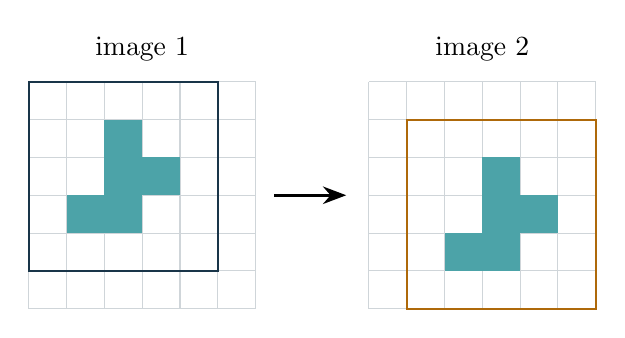
\begin{tikzpicture}[scale=0.48,>=Stealth]
 \draw[step=1,quiet!30] (0,0) grid (6,6);
 \draw[step=1,quiet!30] (9,0) grid (15,6);
 \foreach \x/\y in {1/2,2/2,2/3,3/3,2/4}{
  \fill[teal!70] (\x,\y) rectangle ++(1,1);
  \fill[teal!70] (\x+10,\y-1) rectangle ++(1,1);}
 \draw[thick,ink] (0,1) rectangle (5,6);
 \draw[thick,gold] (10,0) rectangle (15,5);
 \draw[->,very thick] (6.5,3)--(8.4,3);
 \node[above] at (3,6.3) {image 1};
 \node[above] at (12,6.3) {image 2};
 \end{tikzpicture}
 \column{0.35\textwidth}
 \begin{enumerate}
  \item Cut out a template.
  \item Slide a matching window.
  \item Score each shift.
  \item Refine the best peak.
 \end{enumerate}
 \end{columns}
 \takeaway{The measurement uses an entire patch of texture.}
\end{frame}

\evidence{Concrete teaching implementation: src/jiram\_catalog/tracking.py; original Tracker equivalence is unverified.}
\begin{frame}{Correlation compares patterns, with a validity mask}
 \[
 C(\bm d)=\frac{\sum_{i\in M(\bm d)}(A_i-\bar A)(B_i(\bm d)-\bar B)}
 {\sqrt{\sum_{i\in M(\bm d)}(A_i-\bar A)^2
 \sum_{i\in M(\bm d)}(B_i(\bm d)-\bar B)^2}}
 \]
 \begin{itemize}
  \item Means and sums use $M(\bm d)$: pixels valid in both trial patches.
  \item Mean subtraction removes a constant brightness offset.
  \item Normalization removes a positive gain change.
  \item A local peak fit permits a subpixel displacement estimate.
 \end{itemize}
 \takeaway{A gap filled with zero can become a convincing false feature.}
\end{frame}

\evidence{Original optical-flow derivation; an explanatory comparison, not undocumented Tracker internals.}
\begin{frame}{Optical flow begins with a brightness assumption}
 \[
 I(\bm x+\bm v\Delta t,t+\Delta t)\simeq I(\bm x,t)
 \quad\Longrightarrow\quad I_t+uI_x+vI_y\simeq0.
 \]
 \begin{columns}[T]
 \column{0.48\textwidth}
 \textbf{Patch tracking}\par
 Search finite shifts of a neighborhood.
 \column{0.48\textwidth}
 \textbf{Differential optical flow}\par
 Fit brightness derivatives with spatial constraints.
 \end{columns}
 \vspace{0.5cm}
 Both become ambiguous when texture evolves independently of motion:
 \[
 I_t+\bm v\cdot\nabla I=S_I.
 \]
 \takeaway{Cloud formation or radiometric change can be mistaken for advection.}
\end{frame}

\evidence{Original aperture-problem illustration. Arrows are hypothetical motions.}
\begin{frame}{A straight stripe cannot reveal every motion component}
 \begin{columns}[c]
 \column{0.45\textwidth}
 \begin{center}
 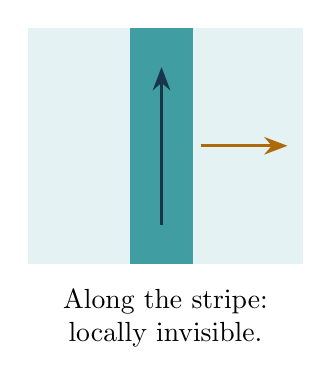
\begin{tikzpicture}[>=Stealth]
 \fill[teal!10] (0,0) rectangle (3.5,3);
 \fill[teal!75] (1.3,0) rectangle (2.1,3);
 \draw[->,very thick,ink] (1.7,0.5)--(1.7,2.5);
 \draw[->,very thick,gold] (2.2,1.5)--(3.3,1.5);
 \node[below,align=center] at (1.75,-0.2) {Along the stripe:\\locally invisible.};
 \end{tikzpicture}
 \end{center}
 \column{0.5\textwidth}
 The brightness equation contains two unknown velocity components.
 \par\medskip
 Texture with gradients in several directions supplies additional constraints.
 \par\medskip
 A smooth or repetitive patch may have many plausible matches.
 \end{columns}
\end{frame}

\evidence{Entropy is a reported quality measure; limitations and extra checks are original analysis/proposals.}
\begin{frame}{Texture quality needs more than one score}
 \begin{columns}[T]
 \column{0.43\textwidth}
 \textbf{Histogram entropy}\par
 \[H=-\sum_{k:p_k>0}p_k\log_2p_k\]
 Uniform patch: low $H$.\par
 Many intensity levels: higher $H$.
 \column{0.53\textwidth}
 \textbf{What it cannot guarantee}\par
 A smooth ramp can have high entropy.\par
 Random noise can have high entropy.\par
 Neither guarantees a unique, persistent match.
 \end{columns}
 \takeaway{Also inspect peak ambiguity, valid area, directional texture and forward/backward consistency.}
\end{frame}

\evidence{Original scale explanation, motivated by the experiment's published sampling and template sizes.}
\begin{frame}{Sampling, support and resolution answer different questions}
 \small
 \begin{tabularx}{\linewidth}{@{}p{3.7cm}X@{}}
 \toprule
 Native sampling & How far apart are detector samples on Jupiter?\\
 Map spacing & How fine is the resampled coordinate grid?\\
 Template support & How large a patch constrains one velocity?\\
 Vector spacing & How far apart do we report estimates?\\
 Derivative scale & Over what area do we measure spin or spreading?\\
 \bottomrule
 \end{tabularx}
 \vspace{0.4cm}
 Interpolating an image or drawing more arrows does not add observations.
 \takeaway{The interface should display these scales separately.}
\end{frame}

\evidence{Original synthetic oversampling example. Diagram depicts one broad support window.}
\begin{frame}{Many arrows can reuse almost the same information}
 \begin{columns}[c]
 \column{0.48\textwidth}
 \begin{center}
 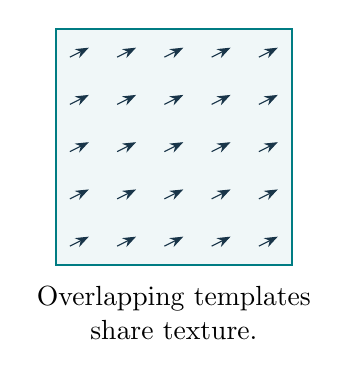
\begin{tikzpicture}[scale=0.6,>=Stealth]
 \fill[teal!6] (0,0) rectangle (5,5);
 \draw[thick,teal] (0,0) rectangle (5,5);
 \foreach \x in {0.5,1.5,2.5,3.5,4.5}{
  \foreach \y in {0.5,1.5,2.5,3.5,4.5}{
   \draw[->,ink] (\x-0.2,\y-0.1)--++(0.4,0.2);}}
 \node[below,align=center] at (2.5,-0.25) {Overlapping templates\\share texture.};
 \end{tikzpicture}
 \end{center}
 \column{0.48\textwidth}
 Synthetic example:\par\medskip
 Useful patch width: 240 km.\par
 Vector spacing: 40 km $\to$ 10 km.\par\medskip
 Sixteen times as many vectors per unit area; no new photons.
 \end{columns}
 \takeaway{Do not count overlapping vectors as independent samples.}
\end{frame}

\evidence{Original Cartesian vector-calculus examples. Positive normal is out of the page.}
\begin{frame}{Vorticity measures spin; divergence measures spreading}
 \begin{columns}[T]
 \column{0.48\textwidth}
 \textbf{Rigid rotation}\par
 \[(u,v)=(-\omega y,\omega x)\]
 \[\zeta=v_x-u_y=2\omega,\qquad D=0\]
 \begin{center}
 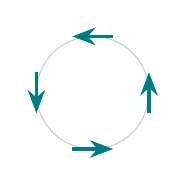
\begin{tikzpicture}[>=Stealth,scale=0.65]
 \draw[quiet!35] (0,0) circle (1.1);
 \foreach \a in {0,90,180,270}{
  \begin{scope}[rotate=\a]\draw[->,very thick,teal] (1.1,-0.4)--(1.1,0.4);\end{scope}}
 \end{tikzpicture}
 \end{center}
 \column{0.48\textwidth}
 \textbf{Isotropic expansion}\par
 \[(u,v)=(\alpha x,\alpha y)\]
 \[\zeta=0,\qquad D=u_x+v_y=2\alpha\]
 \begin{center}
 
\begin{tikzpicture}[>=Stealth,scale=0.65]
 \foreach \a in {0,45,...,315}{
  \draw[->,very thick,gold] (\a:0.35)--(\a:1.35);}
 \end{tikzpicture}
 \end{center}
 \end{columns}
 Both diagnostics have units $\sone$; uniform translation gives zero for both.
\end{frame}

\evidence{Original derivation of the contour principle; exact original quadrature remains unverified.}
\begin{frame}{Measure a region through its boundary}
 \begin{columns}[c]
 \column{0.39\textwidth}
 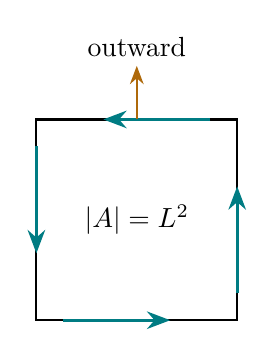
\begin{tikzpicture}[>=Stealth,scale=0.85]
 \draw[thick] (0,0) rectangle (3,3);
 \draw[->,very thick,teal] (0.4,0)--(2,0);
 \draw[->,very thick,teal] (3,0.4)--(3,2);
 \draw[->,very thick,teal] (2.6,3)--(1,3);
 \draw[->,very thick,teal] (0,2.6)--(0,1);
 \draw[->,thick,gold] (1.5,3)--(1.5,3.8);
 \node at (1.5,1.5) {$|A|=L^2$};
 \node[above] at (1.5,3.8) {outward};
 \end{tikzpicture}
 \column{0.59\textwidth}
 \textbf{Circulation / area}\par
 \[\bar\zeta_A=\frac{1}{|A|}\oint(u\,dx+v\,dy)\]
 \textbf{Outward flux / area}\par
 \[\bar D_A=\frac{1}{|A|}\oint(u\,dy-v\,dx)\]
 Counterclockwise contour; physical Cartesian basis.
 \end{columns}
 \takeaway{These are area means. Missing edges must not silently become zero flow.}
\end{frame}

\evidence{Original synthetic uncertainty example; assumes four independent edge-mean errors.}
\begin{frame}{Small velocity errors can overwhelm a derivative}
 \[\sigma_{\bar D}\simeq\sigma_{\bar\zeta}\simeq\frac{2\sigma_e}{L}\]
 \begin{columns}[T]
 \column{0.47\textwidth}
 \textbf{Illustrative assumptions}\par
 Four independent edge means.\par
 Each uncertain by $6.29\,\ms$.\par
 Square side $L=200$ km.
 \column{0.47\textwidth}
 \textbf{Result}\par
 Derivative noise:
 \[6.29\times10^{-5}\,\sone\]
 Larger than a true divergence of
 $2\times10^{-5}\,\sone$.
 \end{columns}
 \takeaway{Real propagation must retain covariance: $\Var(q)=\bm w^T\mathsf C\bm w$.}
\end{frame}

\evidence{Original derivation of a repeat-measurement error model; compare Ingersoll et al., Eqs. 1--2.}
\begin{frame}{Agreement between repeats estimates a common signal}
 \[A=s+e_A,\qquad B=s+e_B\]
 Assume the same physical signal, independent errors, no signal--error
 covariance, and equal individual noise variances.
 \begin{align*}
 \Var(A)=\Var(B)&=\sigma_s^2+\sigma_n^2,\\
 \Cov(A,B)&=\sigma_s^2,\\
 \eta=\operatorname{corr}(A,B)&=\frac{\sigma_s^2}{\sigma_s^2+\sigma_n^2}.
 \end{align*}
 \takeaway{Under this model, correlation is a signal fraction of variance.}
\end{frame}

\evidence{Original synthetic covariance example; numbers are not taken from the Jupiter analysis.}
\begin{frame}{Try the noise calculation with simple numbers}
 Each repeated measurement has standard deviation $10$.\par\medskip
 Their correlation is $0.36$.
 \vspace{0.4cm}
 \begin{columns}[T]
 \column{0.31\textwidth}
 \textbf{Common signal}\par
 \[\sigma_s^2=0.36(10^2)\]
 \[\boxed{\sigma_s=6}\]
 \column{0.31\textwidth}
 \textbf{Individual noise}\par
 \[\sigma_n^2=100-36\]
 \[\boxed{\sigma_n=8}\]
 \column{0.31\textwidth}
 \textbf{Noise after averaging}\par
 \[\sigma_{n,\rm mean}=8/\sqrt2\]
 \[\boxed{\sigma_{n,\rm mean}=5.66}\]
 \end{columns}
 \takeaway{Correlation 0.36 does not mean 36\% of vectors are correct.}
\end{frame}

\evidence{Original assessment of assumptions and shared-image covariance.}
\begin{frame}{A repeatable error can look like repeatable atmosphere}
 \begin{itemize}
 \item \textbf{Shared navigation:} both estimates can inherit the same bias.
 \item \textbf{Changing clouds:} real evolution can lower repeat correlation.
 \item \textbf{Repeated texture failure:} the same ambiguity can fool both pairs.
 \item \textbf{Shared image:} adjacent pairs reuse a position error with opposite signs.
 \end{itemize}
 \small For independent position errors with equal variance $\sigma_p^2$:
 \[
 e_{12}=\frac{p_2-p_1}{\Delta t},\quad
 e_{23}=\frac{p_3-p_2}{\Delta t}
 \ \Rightarrow\ {}
 \Cov(e_{12},e_{23})=-\frac{\sigma_p^2}{\Delta t^2}.
 \]
 \takeaway{Disjoint pairs help; independent physical validation still matters.}
\end{frame}

\evidence{Reported numbers: Ingersoll et al., Table 1 and Methods; interpretation qualified by the error model.}
\begin{frame}{The repeat measurements distinguish stronger and weaker signals}
 \begin{center}
 \begin{tabular}{@{}lcc@{}}
 \toprule
 At a 180 km contour scale & Vorticity & Divergence\\
 \midrule
 Repeat correlation & $\approx0.729$ & $\approx0.299$\\
 \bottomrule
 \end{tabular}
 \end{center}
 \vspace{0.5cm}
 The fitted velocity uncertainty was approximately $7.8\,\ms$ per component.
 \par\medskip
 Under the repeat-measurement model, divergence contains a smaller signal
 fraction than vorticity.
 \takeaway{Velocity, vorticity and divergence need separate confidence assessments.}
\end{frame}

\evidence{Original axisymmetric derivation; the paper reports evidence for anticyclonic shielding.}
\begin{frame}{A shielding ring does not require reversed wind arrows}
 \[\zeta(r)=\frac{1}{r}\frac{d\left(rv_\theta\right)}{dr}\]
 \begin{columns}[T]
 \column{0.47\textwidth}
 Consider a synthetic profile:
 \[v_\theta=Cr^{-p},\qquad C>0.\]
 The azimuthal wind remains positive.
 \column{0.47\textwidth}
 Its vorticity is
 \[\zeta=(1-p)Cr^{-p-1}.\]
 For $p>1$, the vorticity is negative.
 \end{columns}
 \takeaway{Wind decreasing faster than $1/r$ can produce an anticyclonic annulus.}
\end{frame}

\evidence{Publication distinction: Ingersoll et al. (2022); Siegelman et al. (2022), Nature Physics, doi:10.1038/s41567-021-01458-y.}
\begin{frame}{Divergence does not directly measure vertical velocity}
 \[
 \text{Simple incompressible continuity:}\qquad
 D=-\frac{\partial w}{\partial z}.
 \]
 This constrains a vertical gradient. A compressible atmosphere requires
 density and vertical-structure information.
 \par\medskip
 Ingersoll et al. did not detect the proposed divergence--anticyclonic
 vorticity correlation at their resolved scales.
 \par\medskip
 Siegelman et al. used infrared optical-depth anomalies and additional
 surface-quasigeostrophic assumptions to investigate smaller scales.
 \takeaway{A direct wind diagnostic and a model-assisted reconstruction have different assumptions.}
\end{frame}

\evidence{Repository evidence: saved docs/reports/tracking\_pj4.md summaries; not regenerated for this deck.}
\begin{frame}{Our existing tracker is a starting point, with substantial tails}
 \small
 \begin{tabularx}{\linewidth}{@{}Xrrr@{}}
 \toprule
 Comparison input & Median error & 90th percentile & Within 1 px\\
 \midrule
 Published maps & 0.224 px & 4.759 px & 83.4\%\\
 Our reprojections & 0.434 px & 4.685 px & 80.1\%\\
 \bottomrule
 \end{tabularx}
 \normalsize\vspace{0.45cm}
 24 same-letter tile pairs, subsampled reference positions.\par\medskip
 Median vector-difference magnitudes: $3.45$ and $6.69\,\ms$.
 \par\medskip
 These compare with published vectors, not exact atmospheric truth.
 \takeaway{Good median agreement does not establish derivative accuracy.}
\end{frame}

\evidence{Repository evidence: selected TP4 header, tracking.py, reproject.py, regions.py and api/science.py.}
\begin{frame}{Resolve three provenance details before claiming reproduction}
 \begin{enumerate}
 \item \textbf{Software identity:} paper says Tracker3; local table history
 says TRACKER4. Equivalence is unverified.
 \item \textbf{Sampling:} the inspected raw table has \texttt{GRID=1} and
 15 km map pixels. Its placement differs from the reported analysis grid.
 ``45 km'' is not evidence of cloud altitude.
 \item \textbf{Coordinates:} sample/line and map/array axes differ.
 Verify the physical basis before assigning wind directions or curl signs.
 \end{enumerate}
 \takeaway{The GUI currently loads associated vector products; it does not yet supply this complete wind workflow.}
\end{frame}

\evidence{Proposed features. No application implementation or new wind retrieval is part of this documentation task.}
\begin{frame}{Build the next features around inspectable measurements}
 \begin{columns}[T]
 \column{0.31\textwidth}
 \textbf{1. Design the experiment}\par\medskip
 Four-set selector.\par
 Exact source times.\par
 Common valid coverage.\par
 Instrument eligibility.
 \column{0.31\textwidth}
 \textbf{2. Inspect every vector}\par\medskip
 Paired patches.\par
 Correlation surface.\par
 Masks and uncertainty.\par
 Saved source association.
 \column{0.31\textwidth}
 \textbf{3. Test the science}\par\medskip
 Contour-scale control.\par
 Repeatability panel.\par
 Synthetic benchmarks.\par
 Reference comparisons.
 \end{columns}
 \takeaway{Start with a reproducible PJ4 benchmark; then validate other passes and JunoCam.}
\end{frame}

\evidence{Proposed instrument-specific extension; current exclusion and navigation limits: docs/open\_items.md.}
\begin{frame}{JunoCam needs its own motion-validation evidence}
 \begin{itemize}
  \item Retain instrument-failure exclusions and native-band provenance.
  \item Preserve framelet timing, map support and source identity.
  \item Quantify navigation and band-registration errors.
  \item Check reflected-light changes separately from JIRAM thermal texture.
 \end{itemize}
 \takeaway{A regular tensor, clean image or successful export does not establish accurate winds.}
\end{frame}

\evidence{Original learning checkpoint. Answers follow from the synthetic derivations in this deck.}
\begin{frame}{Check your understanding before building anything}
 \begin{enumerate}
  \item Does halving vector spacing necessarily resolve smaller eddies?
  \item Can a constant navigation translation create curl in an ideal plane?
  \item Can two biased estimates correlate almost perfectly?
  \item Does horizontal divergence uniquely determine upward velocity?
 \end{enumerate}
 \vspace{0.5cm}
 \small\textbf{Answers:} No. No---spatially varying errors are different.
 Yes. No---vertical structure is needed.
 \takeaway{Resolution, repeatability and physical accuracy are separate questions.}
\end{frame}

\evidence{Source and reproducibility record. The main article was read in full, including Methods.}
\begin{frame}{Sources and companion notes}
 \small
 \textbf{Main paper}\par
 \paperlink{}, \emph{Vorticity and divergence at scales down to 200 km
 within and around the polar cyclones of Jupiter}.\par
 \href{https://pordlabs.ucsd.edu/wryoung/reprintPDFs/VortDiv.pdf}{Full coauthor-hosted PDF}:
 Methods pp. 1284--1285, Figs. 2--3, Table 1.
 \par\medskip
 \textbf{Related dynamical inference}\par
 \href{https://doi.org/10.1038/s41567-021-01458-y}{Siegelman et al. (2022),
 Moist convection drives an upscale energy transfer at Jovian high latitudes}.
 \par\medskip
 \textbf{Repository and full derivations}\par
 \repolink{}; \texttt{tracking.py}; \texttt{api/science.py}.\par
 Companion: \texttt{docs/pedagogy/ingersoll\_2022\_tracking.tex}.
 \par\medskip
 Original diagrams and synthetic examples; no article figures reproduced.
\end{frame}

\evidence{Judgment calls, access limits and unresolved alternatives.}
\begin{frame}{Judgment calls and what remains unverified}
 \begin{itemize}
  \item Chose a short measurement tutorial, with full derivations in companion
  notes, rather than reproducing the complete vortex-dynamics analysis.
  \item Kept the published recipe, local implementation, original teaching
  examples and proposed features distinct.
  \item Treated reference agreement as a benchmark, not perfect wind truth;
  raw placement and analysis-grid sampling remain separate.
  \item Supplementary methods were inaccessible: the entropy cutoff, exact
  quadrature, raw-to-analysis aggregation and Tracker version equivalence
  remain unverified. No settings were invented to fill those gaps.
 \end{itemize}
 \takeaway{Next implementation requires an accepted specification and scientific validation.}
\end{frame}

\end{document}
